\documentclass[border=10pt]{standalone}
\usepackage{tikz}
\usetikzlibrary{arrows.meta, calc, shapes}

\begin{document}
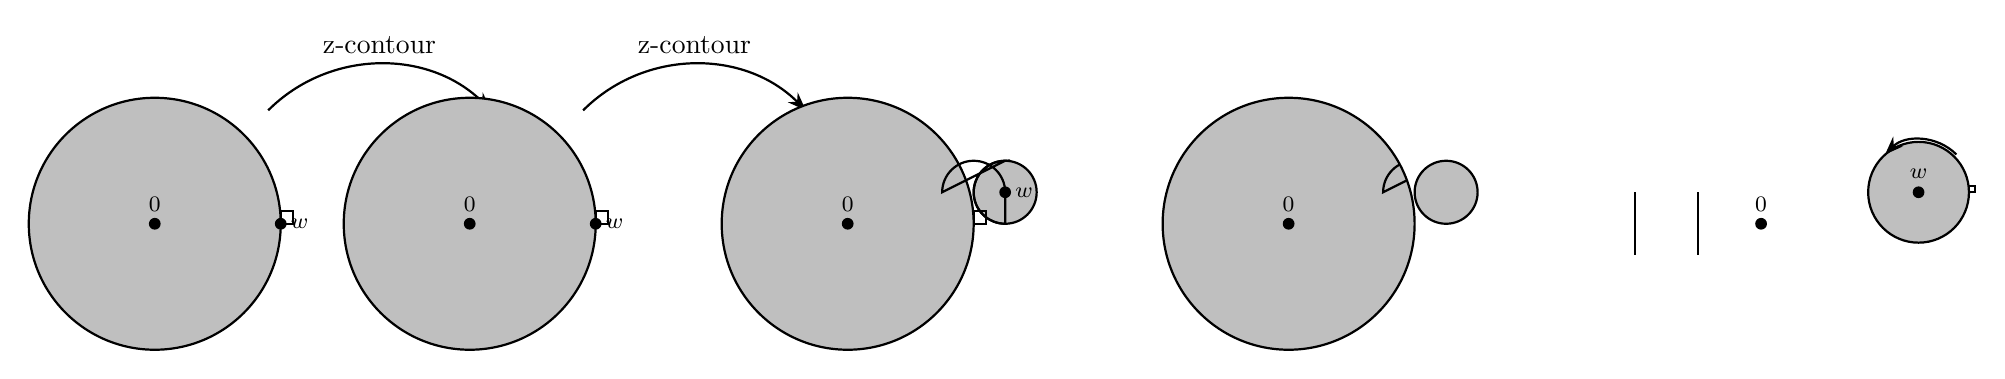
\begin{tikzpicture}[scale=0.8, thick]

% Define styles
\tikzset{
    contour/.style={thick, black, ->, >=Stealth, bend left=45},
    point/.style={fill=black, circle, inner sep=1.5pt},
    region/.style={fill=lightgray, draw=black, thick},
    label/.style={font=\footnotesize, black}
}

% First diagram: disk with w on boundary
\begin{scope}[xshift=0cm]
    \draw[region] (0,0) circle (2);
    \node[point] at (0,0) {};
    \node[label] at (0,0.3) {$0$};
    \node[point] at (2,0) {};
    \node[label] at (2.3,0) {$w$};
    \draw[contour] (1.8,1.8) arc (135:45:2.5) node[midway, above] {z-contour};
    \draw[thick] (2,0) -- (2.2,0) -- (2.2,0.2) -- (2,0.2) -- cycle; % small tick
\end{scope}

% Minus sign
\draw (3.5,0) -- (4.5,0);

% Second diagram: same as first
\begin{scope}[xshift=5cm]
    \draw[region] (0,0) circle (2);
    \node[point] at (0,0) {};
    \node[label] at (0,0.3) {$0$};
    \node[point] at (2,0) {};
    \node[label] at (2.3,0) {$w$};
    \draw[contour] (1.8,1.8) arc (135:45:2.5) node[midway, above] {z-contour};
    \draw[thick] (2,0) -- (2.2,0) -- (2.2,0.2) -- (2,0.2) -- cycle;
\end{scope}

% Arrow
\draw[->, thick] (9.5,0) -- (10.5,0);

% Third diagram: disk with bubble at w
\begin{scope}[xshift=11cm]
    \draw[region] (0,0) circle (2);
    \draw[region] (2.5,0.5) circle (0.5);
    \draw[thick] (2,0) -- (2.2,0) -- (2.2,0.2) -- (2,0.2) -- cycle;
    \node[point] at (0,0) {};
    \node[label] at (0,0.3) {$0$};
    \node[point] at (2.5,0.5) {};
    \node[label] at (2.8,0.5) {$w$};
    \draw[contour] (2.5,1) arc (90:270:0.5) -- (2.5,0.5) arc (0:180:0.5) -- cycle; % contour around bubble
\end{scope}

% Minus sign
\draw (16.5,0) -- (17.5,0);

% Fourth diagram: disk with dent at w
\begin{scope}[xshift=18cm]
    \draw[region] (0,0) circle (2);
    \draw[region] (2.5,0.5) circle (0.5);
    \clip (0,0) circle (2);
    \draw[region] (2.5,0.5) circle (0.5);
    \draw[thick] (2,0) -- (2.2,0) -- (2.2,0.2) -- (2,0.2) -- cycle;
    \node[point] at (0,0) {};
    \node[label] at (0,0.3) {$0$};
    \node[point] at (2.5,0.5) {};
    \node[label] at (2.8,0.5) {$w$};
    \draw[contour] (2.5,1) arc (90:270:0.5) -- (2.5,0.5) arc (0:180:0.5) -- cycle; % contour around dent
\end{scope}

% Equals sign
\draw (23.5,0.5) -- (23.5,-0.5);
\draw (24.5,0.5) -- (24.5,-0.5);

% Fifth diagram: just point 0
\begin{scope}[xshift=25.5cm]
    \node[point] at (0,0) {};
    \node[label] at (0,0.3) {$0$};
\end{scope}

% Small circle with w on the right
\begin{scope}[xshift=28cm, yshift=0.5cm]
    \draw[region] (0,0) circle (0.8);
    \node[point] at (0,0) {};
    \node[label] at (0,0.3) {$w$};
    \draw[contour] (0.6,0.6) arc (45:135:0.8);
    \draw[thick] (0.8,0) -- (0.9,0) -- (0.9,0.1) -- (0.8,0.1) -- cycle;
\end{scope}

\end{tikzpicture}
\end{document}